

%================1.3
\section{Phân tích tương quan và các moment đặc trưng mẫu}

Trong phân tích dữ liệu đa biến, việc nghiên cứu mối quan hệ giữa các biến và mô tả đặc trưng của mẫu đóng vai trò nền tảng. Thông qua các công cụ thống kê như trung bình và vectơ trung bình, ta có thể tóm tắt xu hướng phân bố của dữ liệu cũng như hỗ trợ cho các phương pháp phân tích nâng cao như phân tích tương quan hay phân lớp.

Cho $\bm{X} = (X_1, X_2, \dots, X_d)^T$ là một điểm ngẫu nhiên $d$ chiều. Xét mẫu ngẫu nhiên cỡ $n$ lấy từ $\bm{X}$, ký hiệu bởi $\bm{x}_1, \bm{x}_2, \dots, \bm{x}_{n}$, với $\bm{x}_i \in \mathbb{R}^d$. Ta quan tâm đến các moment đặc trưng sau đây.

%================1.3.1
\subsection{Các mô-men đặc trưng mẫu}

Cho $\bm{x}_{1}, \bm{x}_{2}, \dots, \bm{x}_{n}$ là mẫu thể hiện cỡ $n$ lấy từ vectơ ngẫu nhiên $d$ chiều $\bm{X} = (\bm{X}_1, \bm{X}_2, \dots, \bm{X}_d)^\top$. Ta quan tâm các moment mẫu đặc trưng sau đây.
\begin{itemize}
	\item Điểm (vectơ) trung bình mẫu (the sample mean vector) là vectơ  $d$ chiều xác định bởi
	\begin{equation}
		\overline{\bm{x}} \equiv \frac{1}{n} \sum_{i=1}^{n} \bm{x}_i = \begin{pmatrix} 
			\overline{x}_1 \\ 
			\overline{x}_2 \\ 
			\vdots \\ 
			\overline{x}_d 
		\end{pmatrix},
	\end{equation}
	trong đó
	\begin{equation}
		\overline{x}_j = \frac{1}{n} \sum_{i=1}^{n} x_{ij}
	\end{equation}
	là trung bình mẫu của quan sát trên biến thứ $j$ ($j = 1, 2, \dots, d$).
\end{itemize}


\begin{itemize}
	\item Ma trận hiệp phương sai mẫu (the sample covariance matrix) được xác định như sau
	\begin{equation}
		S = \frac{1}{n-1} \sum_{i=1}^{n} (\bm{x}_i - \overline{x})(\bm{x}_i - \overline{x})^{\top} = 
		\begin{pmatrix}
			s_{11} & s_{12} & \dots & s_{1d} \\
			s_{21} & s_{22} & \dots & s_{2d} \\
			\vdots & \vdots & \ddots & \vdots \\
			s_{d1} & s_{d2} & \dots & s_{dd}
		\end{pmatrix},
	\end{equation}
	ở đây 
	\begin{equation}
		s_{jk} = \frac{1}{n-1} \sum_{i=1}^{n} (x_{ij} - \overline{x}_j)(x_{ik} - \overline{x}_k)
	\end{equation}
	là hiệp phương sai mẫu của hai biến thứ $j$ và thứ $k$, và 
	\begin{equation}
		s_{jj} = \frac{1}{n-1} \sum_{i=1}^{n} (x_{ij} - \overline{x}_j)^2
	\end{equation}
	là phương sai mẫu của biến thứ $j$.
\end{itemize}

\subsection{Hệ số tương quan mẫu}

Hiệp phương sai cung cấp thông tin về xu hướng biến thiên đồng thời giữa các biến ngẫu nhiên, tuy nhiên đại lượng này phụ thuộc vào thang đo của từng biến nên khó sử dụng để so sánh mức độ liên hệ giữa các cặp biến khác nhau.

Do đó, cần xây dựng một đại lượng chuẩn hóa từ hiệp phương sai, không phụ thuộc vào đơn vị đo, nhằm phản ánh chính xác mức độ và chiều hướng của mối quan hệ tuyến tính giữa các biến. Đại lượng đó chính là hệ số tương quan.

Với $\bm{x}_1, \bm{x}_2, \dots, \bm{x}_n$ là mẫu thể hiện cỡ $n$ được lấy từ vectơ ngẫu nhiên $d$ chiều $\bm{X} = (X_1, X_2, \dots, X_d)^T$, và đặt $X_j^*$ là biến ngẫu nhiên mẫu ứng với biến $X_j$ ($j=\overline{1,d}$), nghĩa là 
\begin{equation*}
	P(X_j^*=x_{ij}) = \frac{1}{n}, \quad \forall i= 1,2,\dots,n
\end{equation*} Khi đó, hệ số tương quan mẫu giữa hai biến thứ $j$ và thứ $k$ (ký hiệu $r_{jk}$) được xác định là hệ số tương quan giữa hai biến $X_j^*$ và $X_k^*$

\begin{equation}
	\begin{aligned}
		r_{jk}=\rho_{X_j^*, X_k^*} &= \frac{\text{cov}(X_j^*, X_k^*)}{\sqrt{D(X_j^*)D(X_k^*)}} \\
		&= \frac{s_{jk}}{\sqrt{s_{jj} s_{kk}}} = \frac{\sum_{i=1}^n (x_{ij} - \overline{x}_j)(x_{ik} - \overline{x}_k)}{\sqrt{\sum_{i=1}^n (x_{ij} - \overline{x}_j)^2} \sqrt{\sum_{i=1}^n (x_{ik} - \overline{x}_k)^2}} .
	\end{aligned}
	\label{eq:1.8}
\end{equation}

\hspace*{0.5cm}Để thấy được ý nghĩa hình học của hệ số tương quan mẫu $r_{jk}$, ta xét một không gian con đặc biệt được sinh bởi vectơ toàn phần tử bằng 1. Không gian này đóng vai trò quan trọng trong việc xác định hướng chiếu và diễn giải ý nghĩa của các phép biến đổi tuyến tính.

Xét không gian vectơ $\mathbb{R}^n$ với tích vô hướng Euclid của hai vectơ $\bm{x} = (x_1, x_2,\dots,x_n)^T$, $\bm{y} = (y_1, y_2,\dots,y_n)^T$ được xác định bởi công thức
$$
\langle \bm{x}, \bm{y} \rangle = \sum_{i=1}^n x_i y_i.
$$
Với tích vô hướng trên, độ dài (chuẩn) của một vectơ $\bm{x} \in \mathbb{R}^n$ được ký hiệu và cho bởi
$$
\|\bm{x}\| = \sqrt{\langle \bm{x}, \bm{x} \rangle} = \sqrt{\sum_{i=1}^n x_i^2}.
$$
Đồng thời, cosin của góc giữa hai vectơ $\bm{x}, \bm{y}$ cũng được xác định như sau
$$
\cos(\bm{x}, \bm{y}) = \frac{\langle \bm{x}, \bm{y} \rangle}{\|\bm{x}\| \|\bm{y}\|}.
$$
Và $\bm{x}$, $\bm{y}$ được gọi là vuông góc với nhau, ký hiệu $\bm{x} \perp \bm{y}$, nếu như 
$$
\cos(\bm{x}, \bm{y}) = 0 \iff \langle \bm{x}, \bm{y} \rangle = 0.
$$
Khi đó, ứng với $\mathbf{1} = (1, 1,\dots,1)^T \in \mathbb{R}^n$, không gian con sinh bởi vectơ này được cho bởi
$$
\langle \mathbf{1} \rangle = \{\alpha \mathbf{1} \mid \alpha \in \mathbb{R}\}.
$$

Không gian $\langle \mathbf{1} \rangle$ biểu diễn đường phân giác thứ nhất hay đường phân giác chính trong hệ trục $\{e_i\}_{i=\overline{1,n}}$, là hệ trục vuông góc chính tắc của $\mathbb{R}^n$. Nói cách khác, vectơ $\mathbf{1}$ tạo với các vectơ đơn vị $e_i$ những góc bằng nhau, do đó $\langle \mathbf{1} \rangle$ chính là không gian sinh bởi vectơ chỉ phương của đường chéo chính trong $\mathbb{R}^n$. Từ cách diễn giải hình học trên, ta có thể xét phép chiếu trực giao của một vectơ bất kỳ lên không gian con $\langle \mathbf{1} \rangle$. Cụ thể, hình chiếu trực giao của vectơ $x_j^*$ lên $\langle \mathbf{1} \rangle$, kí hiệu $\text{proj}_{\mathbf{1}} x_j^*$, với $\bm{x}_j^* = (x_{1j},x_{2j},\dots,x_{nj})^T$ được cho bởi hình sau

\begin{figure}[H]
	\centering
	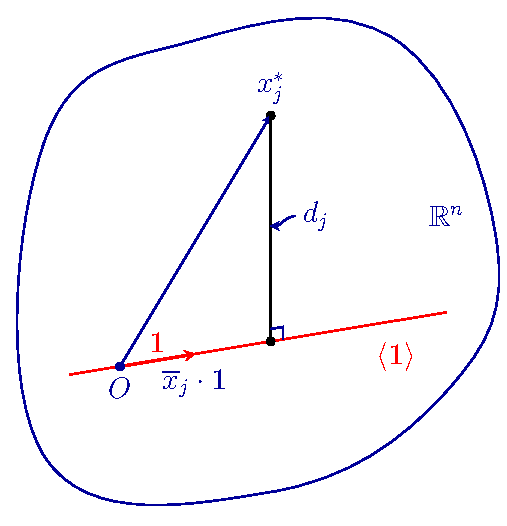
\includegraphics{image/phep_chieu_2.pdf}
	\caption{Hình chiếu trực giao của $\bm{x}_j^*$ lên $\langle \mathbf{1} \rangle$}
	\label{fig:phep_chieu_2}
\end{figure}

Ta chỉ ra $\text{proj}_{\mathbf{1}} \bm{x}_j^* = \overline{x}_j \cdot \mathbf{1}$. Thực vậy, ta có
$$
\begin{aligned}
	\text{proj}_{\mathbf{1}} \bm{x}_j^* 
	&= \|\bm{x}_j^*\| \cos(\bm{x}_j^*, \mathbf{1}) \cdot \frac{\mathbf{1}}{\|\mathbf{1}\|} \\
	&= \|\bm{x}_j^*\| \frac{\langle \bm{x}_j^*, \mathbf{1} \rangle}{\|\bm{x}_j^*\| \|\mathbf{1}\|} \cdot \frac{\mathbf{1}}{\|\mathbf{1}\|} \\
	&= \frac{\langle \bm{x}_j^*, \mathbf{1} \rangle}{\|\mathbf{1}\|^2} \cdot \mathbf{1} \\
	&= \left( \frac{1}{n} \sum_{i=1}^n x_{ij} \right) \cdot \mathbf{1} \\
	&= \overline{x}_j \cdot \mathbf{1}.
\end{aligned}
$$ Vectơ $d_j=\bm{x}_j^*-\overline{x}_j\cdot \mathbf{1} \quad (j =1,2,\dots,d)$ được gọi là vectơ độ lệch của $x_j^*$ đối với $\langle\mathbf{1}\rangle$.

Bước tiếp theo, với hai vectơ $x_j^*$ và $x_k^*$, ta thực hiện phép chiếu (trực giao) của các vectơ này lên $\langle\mathbf{1}\rangle$. (Xem hình \ref{fig:hilbert_3})

\begin{figure}[H]
	\centering
	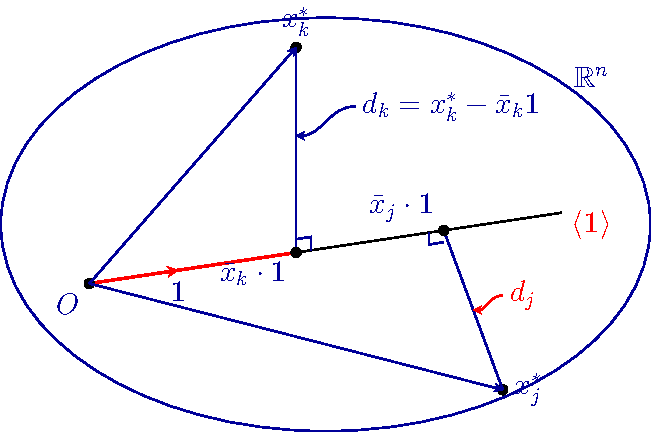
\includegraphics{image/hilbert_3.pdf}
	\caption{Hình chiếu trực giao của hai vectơ $\bm{x}_j^*$, $\bm{x}_k^*$ lên $\langle\mathbf{1}\rangle$}
	\label{fig:hilbert_3}
\end{figure} Đặt, 
$$
\begin{aligned}
	S_j &\equiv \langle \mathbf{1} ,\bm{x}_j^*\rangle = \{\alpha \mathbf{1}+\beta \bm{x}_j^* \mid \alpha,\beta \in \mathbb{R} \}; \\
	S_k &\equiv \langle \mathbf{1}, \bm{x}_k^* \rangle = \{\alpha \mathbf{1}+\beta \bm{x}_k^* \mid \alpha,\beta \in \mathbb{R} \}
\end{aligned}
$$ lần lượt là các mặt phẳng (không gian con) được sinh ra bởi vectơ $\mathbf{1}$ và vectơ $\mathbf{1}$ và một trong hai vectơ $\bm{x}_j^*$ hoặc $\bm{x}_k^*$. Khi đó, cosin giữa góc tạo bởi hai mặt phẳng trên được xác định như sau
$$
\begin{aligned}
	\cos(S_j, S_k) = \cos(\bm{d}_j, \bm{d}_k) \\
	&= \frac{\langle \bm{d}_j, \bm{d}_k \rangle}{\|\bm{d}_j\| \|\bm{d}_k\|} \\
	&= \frac{\sum_{i=1}^n (x_{ij}-\overline{x}_j)(x_{ik}-\overline{x}_k)}{\sqrt{\sum_{i=1}^n(x_{ij}-\overline{x}_j)^2}\sqrt{\sum_{i=1}^n(x_{ik}-\overline{x}_k)^2}} \\
	&= r_{jk}.
\end{aligned}
$$ Ở đây, $d_j = \bm{x}_j^* - \overline{x}_j \cdot \mathbf{1}$ và $d_k = \bm{x}_k^* - \overline{x}_k \cdot \mathbf{1}$ là các vectơ độ lệch của $\bm{x}_j^*$ và $\bm{x}_k^*$ đối với $\langle\mathbf{1}\rangle$.
Bằng việc sử dụng bất đẳng thức Cauchy-Schwarz cho tích vô hướng, có thể thấy 
$$
\begin{aligned}
	|r_{jk}| = 1 &\iff \bm{d}_j = b \bm{d}_k \quad (b \in \mathbb{R}) \\
	&\iff \bm{x}_j^* - \overline{x}_j \mathbf{1} = b(\bm{x}_k^* - \overline{x}_k \mathbf{1}) \\
	&\iff \bm{x}_j^* = b\bm{x}_k^* + a \mathbf{1} \quad (a = \overline{x}_j - b\overline{x}_k).
\end{aligned}
$$ Tức, $\bm{x}_j^* \in S_k$ hay $S_j \equiv S_k$. Điều này nghĩa là có một liên hệ tuyến tính thực sự giữa hai vectơ $\bm{x}_j^*$ và $\bm{x}_k^*$. Khi $r_{jk}=-1$ thì sự phụ thuộc tuyến tính của các giá trị $x_{ij}$ và $x_{ik}$ là nghịch biến và $r_{jk}=1$ thì sự phụ thuộc này là đồng biến.

Ngược lại, khi $r_{jk}=0$, tức $\bm{d}_k \perp \bm{d}_j$ (hay $S_j \perp S_k$) thì mối liên hệ tuyến tính giữa $\bm{d}_j$ và $\bm{d}_k$ là kém hiệu quả nhất. Lúc này, ta nói $\bm{x}_j^*$ và $\bm{x}_k^*$ là không có tương quan tuyến tính với nhau. 

Đồ thị đám mây điểm biểu diễn mức độ tương quan (tuyến tính) của hai vectơ $\bm{x}_j^*$ và $\bm{x}_k^*$ được cho trong hình sau

\begin{figure}[H]
	\centering
	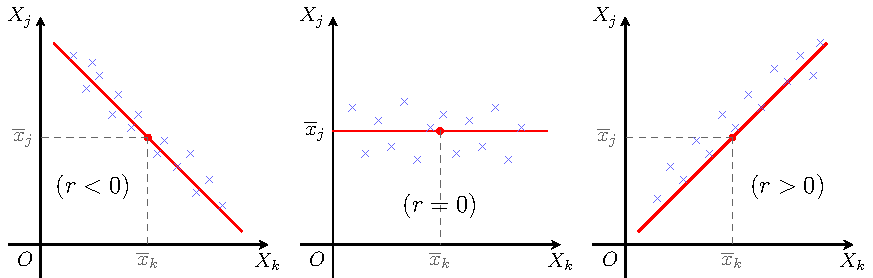
\includegraphics{image/tuongquan.pdf}
	\caption{Đồ thị đám mây điểm biểu diễn mức độ tương quan của hai vectơ $\bm{x}_j^*$ và $\bm{x}_k^*$}
	\label{fig:tuongquan}
\end{figure}


\subsection{Ma trận tương quan mẫu và hệ số tải}
Từ dữ liệu thống kê cỡ $n$ được lấy từ vectơ ngẫu nhiên $d$ chiều $\bm{X} = (X_1,\dots,X_d)^T$, cho trong bảng \ref{tab:raw_data}, ta định nghĩa ma trận tương quan mẫu $\mathbf{r}$ ứng với bộ dữ liệu trên được xác định như sau
\begin{equation}
	\bm{r}= 
	\begin{bmatrix}
		1 & r_{12} & \cdots & r_{1d} \\
		r_{21} & 1 & \cdots & r_{2d} \\
		\vdots & \vdots & \ddots & \vdots \\
		r_{d1} & r_{d2} & \cdots & 1
	\end{bmatrix}, 
	\label{eq:1.9}
\end{equation} với $r_{jk}$ là hệ số tương quan mẫu giữa biến thứ $j$ và biến thứ $k$ được cho trong \ref{eq:1.8} $(j,k = 1,2,\dots,d)$. Do $r_{jk}=r_{kj}$ nên ma trận $\bm{r}$ là đối xứng. Hơn nữa, do tính chất của tương quan mẫu, ta có $r_{jk}=r_{k,j}$ với mọi $k,j=1,2,\dots,d$ nên $\bm{r}$ là ma trận đối xứng. Lưu ý rằng, nếu đặt $\bm{d}_j^*$ ($j=1,2,\dots,d$) là vectơ chuẩn hóa của $\bm{d}_j$, nghĩa là
\begin{equation*}
	\bm{d}_j^*=\frac{\bm{d}_j}{\|\bm{d}_j\|},
\end{equation*} thì $\|\bm{d}_j^*\|=1$ và
\begin{equation}
	\begin{aligned}
		r_{jk} &= \cos(\bm{d}_j, \bm{d}_k) = \frac{\langle \bm{d}_j, \bm{d}_k \rangle}{\|\bm{d}_j\| \|\bm{d}_k\|} \\
		&= \left\langle \frac{\bm{d}_j}{\|\bm{d}_j\|}, \frac{\bm{d}_k}{\|\bm{d}_k\|} \right\rangle \\
		&= \cos(\bm{d}_j^*, \bm{d}_k^*). 
	\end{aligned}
	\label{eq:1.10}
\end{equation}
Một điểm cần chú ý ở đây, khi áp dụng các công cụ thống kê vào thực tế, thông thường thang đo thứ nguyên của các biến $X_j$, $(j=1,2,\dots,d)$ là khác nhau. Do vậy để phản ánh chính xác mối tương quan giữa biến $X_j$ và tổng thể trên dữ liệu mẫu ta cần sử dụng đến hệ số tải (loading factor) cho $X_j$. Đặt,
\begin{align*}
	F &= \bm{d}_1^* + \bm{d}_2^* + \dots + \bm{d}_d^* \\
	&= \sum_{j=1}^d \bm{d}_j^*
\end{align*} là vectơ tổng hợp lực của $d$ vectơ $\bm{d}_j^*$. Hệ số tải ứng với biến $X_j$ (trên dữ liệu mẫu) được cho bởi cosin của góc giữa vectơ $\bm{d}_j^*$ với vectơ tổng hợp lực $F$. Tức là, với $\theta_j = \widehat{(\bm{d}_j^*, F)}$
\begin{equation*}
	\cos(\theta_j) = \cos(\bm{d}_j^*, F).
\end{equation*}
Từ ma trận tương quan mẫu được cho trong \ref{eq:1.9}, hệ số tải ứng với biến $X_j$ được xác định như sau
\begin{equation*}
	\cos(\theta_j) = \frac{\text{Tổng cột | hàng } j \text{ của ma trận } \bm{r}}{\sqrt{\text{Tổng các số hạng của ma trận } \bm{r}}}.
\end{equation*} Thực vậy,
\begin{align*}
	\cos(\theta_j) &= \cos(\bm{d}_j^*, F) \\
	&= \frac{\langle \bm{d}_j^*, F \rangle}{\|\bm{d}_j^*\| \|F\|}.
\end{align*} Ta có,
\begin{align*}
	\langle \bm{d}_j^*, F \rangle &= \left\langle d_j^*, \sum_{k=1}^d d_k^* \right\rangle \\
	&= \sum_{k=1}^d \langle d_j^*, d_k^* \rangle \\
	&= \sum_{k=1}^d r_{jk} \quad \text{(theo~\eqref{eq:1.10})}\\
	&= \text{Tổng cột | hàng $j$ của ma trận $\bm{r}$}
\end{align*} Hơn nữa,
\begin{align*}
	\|F\|^2 &= \langle \sum_{j=1}^d d_j^*,F \rangle\\
	&= \langle \sum_{j=1}^d d_j^*,\sum_{k=1}^d d_k^* \rangle\\
	&= \sum_{j=1}^d\langle d_j^*, F \rangle\\
	&= \text{Tổng các số hạng của ma trận $r$}.
\end{align*} Vì thế,
\begin{equation*}
	\cos(\theta_j) = \frac{\text{Tổng cột | hàng $j$ của ma trận $\bm{r}$}}{\sqrt{\text{Tổng các số hạng của ma trận $\bm{r}$}}}.
\end{equation*} Trực quan hóa hệ số tải trong trường hợp $d=2$ được cho bởi hình sau
\begin{figure}[H]
	\centering
	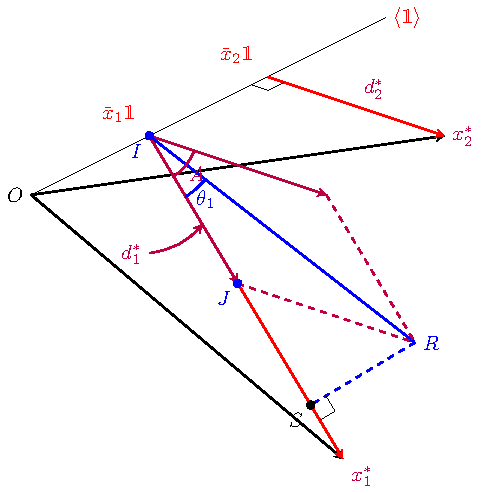
\includegraphics[width=0.7\linewidth]{image/vector_loading_x1.pdf}
	\caption{Minh họa hình học cho hệ số tải}
	\label{fig:vector_angles}
\end{figure}
Để minh họa cho cách xác định hệ số tải, ta xét ví dụ sau

\textbf{Trường hợp} $d = 3$. Xét trường hợp có ba biến $X_1, X_2, X_3$. Khi đó, ta có ba vectơ sai lệch chuẩn hoá
\[
d_1^*, \quad d_2^*, \quad d_3^*.
\]
Gọi $R$ là vectơ tổng hợp của ba vectơ này
\[
R = d_1^* + d_2^* + d_3^*.
\]
Hệ số tải của biến $X_i$ trên vectơ tổng hợp $R$ được xác định bởi cosin của góc giữa $d_i^*$ và $R$
\[
a_i = \cos \theta_i = \cos(d_i^*, R).
\]
Theo định nghĩa cosin giữa hai vectơ
\[
\cos \theta_i = \frac{d_i^{*T} R}{\|d_i^*\| \|R\|}.
\]
Vì $d_i^*$ đã được chuẩn hoá nên
\[
\|d_i^*\| = 1.
\]
Do đó
\[
a_i = \cos \theta_i = \frac{d_i^{*T} R}{\|R\|}.
\]
Với $R = d_1^* + d_2^* + d_3^*$, ta có
\[
a_1 = \frac{1 + r_{12} + r_{13}}{\|R\|},
\]
\[
a_2 = \frac{r_{21} + 1 + r_{23}}{\|R\|},
\]
\[
a_3 = \frac{r_{31} + r_{32} + 1}{\|R\|}.
\]
Như vậy, tử số của mỗi hệ số tải chính là tổng các phần tử trên hàng tương ứng của ma trận tương quan. Tổng quát, với $d$ biến
\[
a_i = \frac{\sum_{j=1}^d r_{ij}}{\|R\|}.
\]
Trong đó,
\[
R = \sum_{j=1}^d d_j^*.
\]
Độ dài của vectơ tổng hợp $R$ được xác định bởi
\[
\|R\|^2 = \sum_{i=1}^d \sum_{j=1}^d r_{ij}.
\]
Do đó
\[
\|R\| = \sqrt{\sum_{i=1}^d \sum_{j=1}^d r_{ij}}.
\]
Suy ra công thức tổng quát của hệ số tải là
\[
\boxed{ a_i = \cos \theta_i = \frac{\sum_{j=1}^d r_{ij}}{\sqrt{\sum_{i=1}^d \sum_{j=1}^d r_{ij}}} }.
\]
Áp dụng với ma trận tương quan đã cho
\[
R = \begin{pmatrix}
	1 & 0,9659 & 0,2588 \\
	0,9659 & 1 & 0,5000 \\
	0,2588 & 0,5000 & 1
\end{pmatrix},
\]
ta có
\[
r_{12} = 0,9659, \qquad r_{13} = 0,2588, \qquad r_{23} = 0,5000.
\]
Tổng tất cả các phần tử trong ma trận tương quan là
\[
\sum_{i=1}^3 \sum_{j=1}^3 r_{ij} = 3 + 2(r_{12} + r_{13} + r_{23}).
\]
Thay số
\[
\sum_{i=1}^3 \sum_{j=1}^3 r_{ij} = 3 + 2(0,9659 + 0,2588 + 0,5000) = 6,4494.
\]
Do đó
\[
\|R\| = \sqrt{6,4494} \approx 2,5396.
\]
Hệ số tải của từng biến là
\[
a_1 = \frac{1 + 0,9659 + 0,2588}{\sqrt{6,4494}} = \frac{2,2247}{2,5396} \approx 0,8760,
\]
\[
a_2 = \frac{0,9659 + 1 + 0,5000}{\sqrt{6,4494}} = \frac{2,4659}{2,5396} \approx 0,9710,
\]
\[
a_3 = \frac{0,2588 + 0,5000 + 1}{\sqrt{6,4494}} = \frac{1,7588}{2,5396} \approx 0,6926.
\]
Vì $a_i = \cos \theta_i$, ta có
\[
\theta_1 = \arccos(0,8760) \approx 28^\circ 50' 11,23''.
\]
\[
\theta_2 = \arccos(0,9710) \approx 13^\circ 49' 55,98''.
\]
\[
\theta_3 = \arccos(0,6926) \approx 46^\circ 9' 49,41''.
\]
Như vậy
\[
a_2 > a_1 > a_3,
\]
hay tương đương
\[
\theta_2 < \theta_1 < \theta_3.
\]
Điều này cho thấy biến $X_2$ có mức độ liên hệ mạnh nhất với trục tổng hợp $R$, vì hệ số tải của $X_2$ là lớn nhất và góc giữa $d_2^*$ với $R$ là nhỏ nhất. Ngược lại, $X_3$ có hệ số tải nhỏ nhất nên có mức độ đại diện yếu hơn cho xu hướng chung của nhóm biến.
